\documentclass{article}
\usepackage[utf8]{inputenc}

\title{LSTM for stock price prediction}
\author{Eytan Ohana 803422, Dean Meyer 802794}
\date{Submitted as final project report for Deep Learning, IDC, 2019}

\usepackage{natbib}
\usepackage{graphicx}
\usepackage{subfig}

\graphicspath{ {./images/} }

\begin{document}

\maketitle

\section{Introduction}

Stock price prediction is the act of trying to determine the future value of a company’s stock based on multitude of inputs. This paper explores the power of using LSTM and its ability to keep and forget information in order to predict stock price successfully. After training the model, our goal was to be able to accurately predict the price of a stock for the following day. As input features, we use a given stock’s daily pricing data (open, high, low, close and volume) and our label is the next day’s stock price. Furthermore, after testing we decided that the sequence length (how many days we look back) should be 100. The proposed model was applied and evaluated using both apple stock (AAPL) and S\&P500 ETF (SPY). We implemented three different models all based on the LSTM infrastructure which will be extrapolated on later. Our best model’s performance gave us an average testing error of 0.14, and is able to capture the trend for the next day.

\subsection{Related Works}

\begin{enumerate}
    \item https://www.jessicayung.com/lstms-for-time-series-in-pytorch/
    \item http://colah.github.io/posts/2015-08-Understanding-LSTMs/
\end{enumerate}




\section{Solution}
\subsection{General approach}
Our approach is to use widely available daily (open, high, low, close, volume) stock information to train some variant of an LSTM neural network to predict trends in the closing price of a stock for the next day. We plan to start out with a simple single layer LSTM then see how our model is affected by adding more LSTM layers or more linear layers.

\subsection{Design}

Our code contains 3 classes of the different architectures we implemented. The following architectures are:
\begin{enumerate}
    \item The first and simplest class is just a single LSTM cell with a single fully connected layer for the output. The main challenge was figuring out a good sequence length to train our model. We ended up settling on 100. The maximum number of training epochs we ran were 50 epochs which took approximately 50 minutes. 
    
    \item The second architecture uses a fully connected single layer to accept the sequence as input and feeds its output into the LSTM which then feeds its output into a final linear layer for output. This network was trained on 30 epochs and gave the best results. After researching online we found that adding a linear layer before the LSTM in order to encode some more information that will be fed into the LSTM.
    
    \item The third network feeds the input through two LSTM's and then feeds the output through a linear layer. This gave the worst results which was surprising as we expected the more "advanced" network to perform better. 
\end{enumerate}


\section{Experimental results}

We evaluated the models based on two metrics:
\begin{enumerate}
    \item Visually, how well they were able to capture the trend of the overall stock price over an entire year by measuring its predicted stock prices to the actual prices in our test set.
    
    \item Based on the mean absolute error (MAE) of the predicted prices and the real prices which measures the average difference between two continuous variables. $$MAE = \frac{1}{m}\sum_{i=1}^{m}|y-\hat{y}|$$
\end{enumerate}

The first model was able to capture trends really well and after training for 30 epochs achieved a MAE of 0.206. After 50 epochs it lowered to 0.191. \\


\begin{center}
	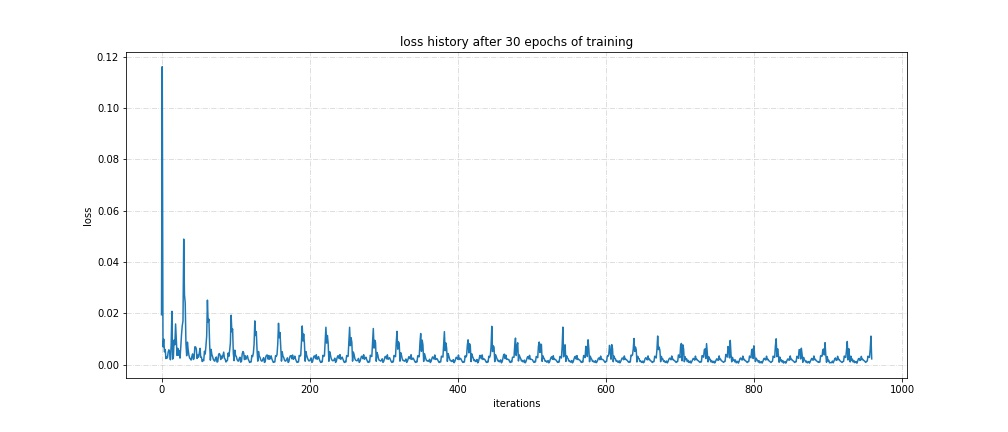
\includegraphics[width=.4\textwidth,height=.25\textwidth]{30-epoch-loss}
	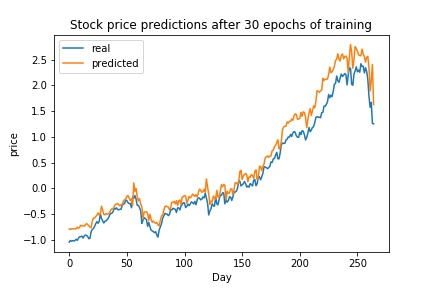
\includegraphics[width=.4\textwidth]{30-epoch-preds}

	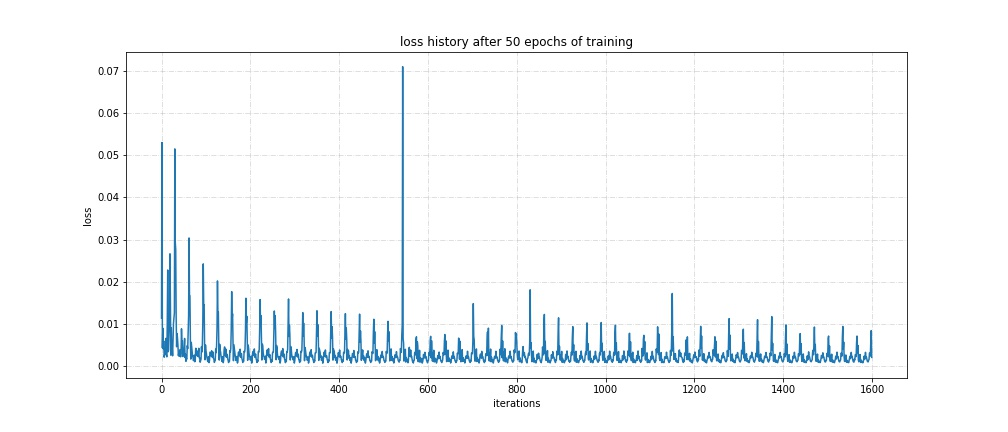
\includegraphics[width=.4\textwidth,height=.25\textwidth]{50-epoch-loss}
	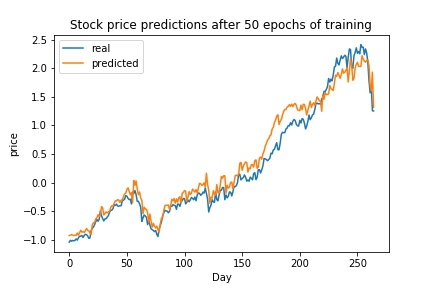
\includegraphics[width=.4\textwidth]{50-epoch-preds}
\end{center}

The second model which contained a Linear layer before and after the LSTM gave the best MAE and was also able to capture the trend really well after 30 epochs of training. We call it the best since it had the best MAE of 0.14

\begin{center}
	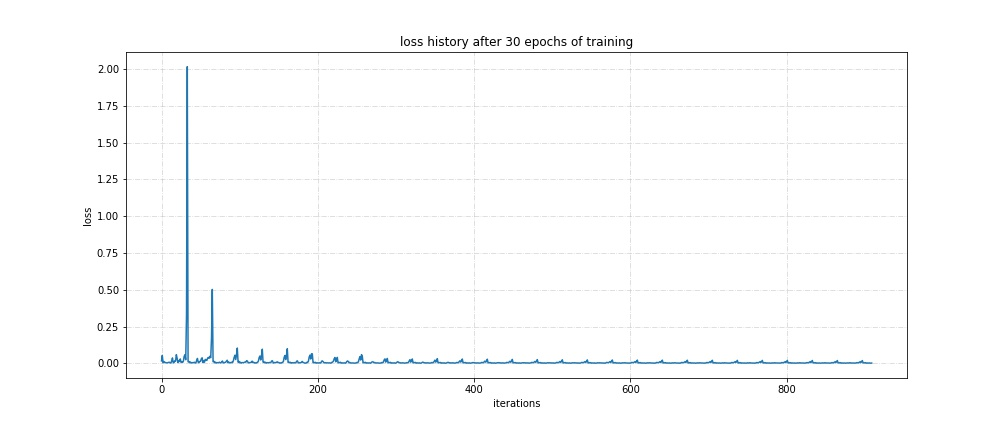
\includegraphics[width=.4\textwidth,height=.25\textwidth]{Linear_first_30-epoch-loss}
	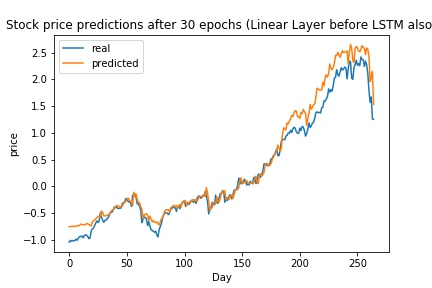
\includegraphics[width=.4\textwidth]{Linear_first_30-epoch-preds1}
\end{center}


The last model made of two LSTM cells connected gave the worst results. It was unable to capture the trend and had the highest MAE 0.637. The model was originally trained on three epochs and gave un-encouraging results which were then confirmed after training for 10 epochs which yielded an MAE of 1.77. 

\begin{center}
	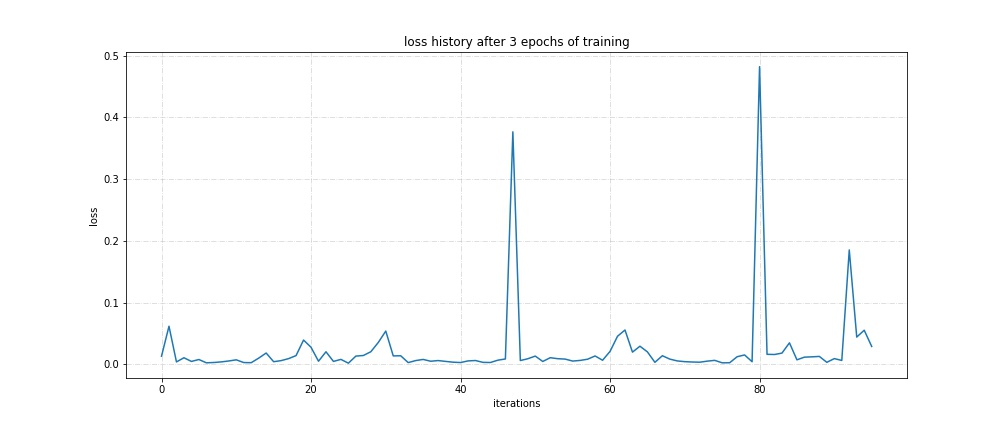
\includegraphics[width=.4\textwidth,height=.25\textwidth]{2-layer-lstm-loss}
	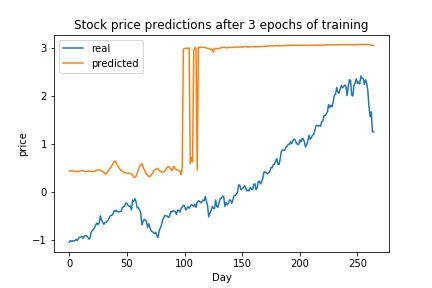
\includegraphics[width=.4\textwidth]{2-layer-lstm-preds}
		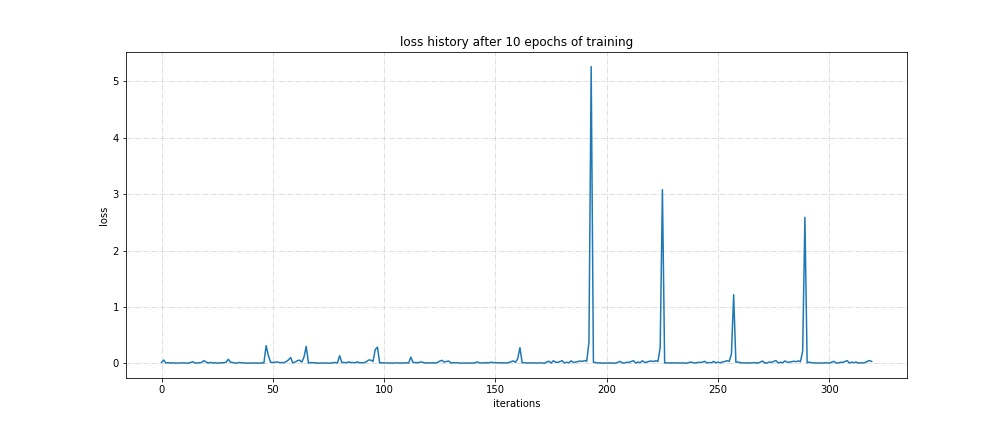
\includegraphics[width=.4\textwidth,height=.25\textwidth]{2-layer-lstm-loss-10-epochs}
	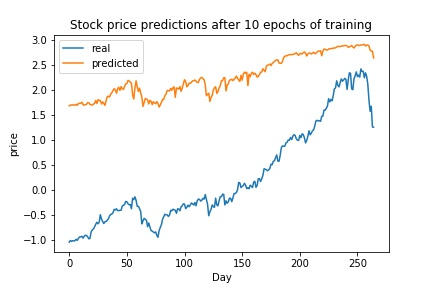
\includegraphics[width=.4\textwidth]{2-layer-lstm-preds-10-epoch}
\end{center}



\section{Discussion}

We chose to try and predict stock pricing and capture trends because we felt it was a worthy goal. Algorithmic trading has been a huge part of financial-trading and trying to predict the market has been a goal for many years now. 

We chose to use LSTM since it's known to perform well on time-series data. Of course we started out with a simple LSTM for a baseline that actually performed pretty well. We then chose to add a linear layer before the LSTM to make the network deeper to hopefully improve it, which turned out to be correct. Finally we thought adding more LSTMs would be even better, but in practice the network performs even worse. 

We also noticed in all of the loss curves there is a distinctive pattern. The first two models have distinct spikes in regular intervals. As the number of iterations increase, we can see that the height of the spikes tends to decrease which is encouraging but we're still not definitively sure why this happens. Upon inspection, the spikes start toward the end of an epoch and decrease until the middle of the next epoch where the loss starts to spike again.

The loss curves for the last model give surprising results too. The spikes don't seem to be decreasing in height but in between the spikes the loss seems pretty stable. Again we're unsure how to interpret this but it is a surprising result. 




\section{Code}

Please provide a link to your code repository. It can be either a Github repository either a colab notebook with additional links for the data.
Good luck!!

Good luck!!
%\bibliographystyle{plain}
%\bibliography{references}
\end{document}
